\section{Logistisches Wachstum}
\begin{code}
	\caption{Skript für die kontinuierliche Berechnung des Verlaufs}
	\mSourceFile{\srcDir/logisticFlys.m}
	\label{source:3-script}
\end{code}
\ \newpage
\begin{figure}[h]
	\centering
	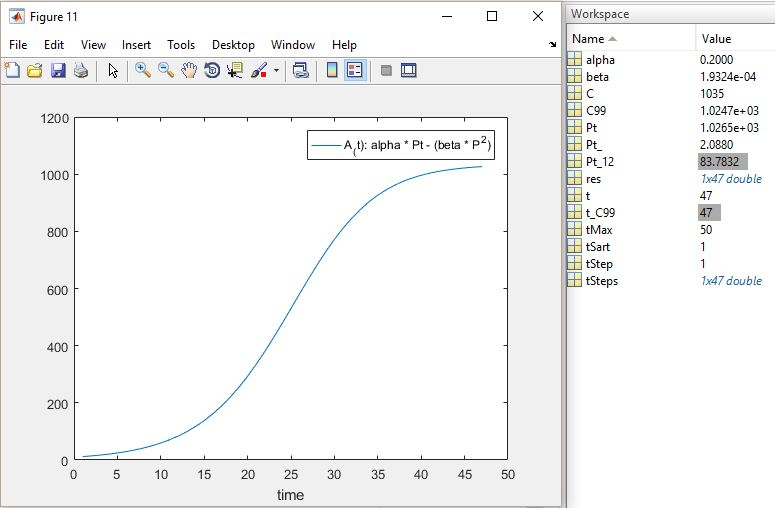
\includegraphics[scale=1,angle=90]{\imageDir/3-test.JPG}
	\caption{t\_99=47, Pt\_12=83.7832}
	\label{fig:3-test}
\end{figure}